\documentclass{article}

\usepackage{Sweave}
\begin{document}
\Sconcordance{concordance:ejemplo.tex:ejemplo.Rnw:%
1 13 1 1 0 40 1 1 2 13 0 1 2 7 1}


\title{ejemplo}
\author{omarpbrasta }
\date{September 2023}

\maketitle

\section{Introduction}
\subsection{HOLA2}
\subsubsection{HOLA 3}

\begin{figure}[h]
    \centering
    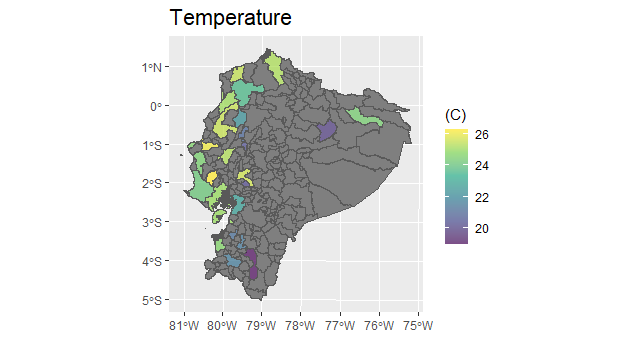
\includegraphics{Rplot.png}
    \caption{Caption}
    \label{fig:enter-label}
\end{figure}


\begin{Schunk}
\begin{Sinput}
> summary(cars)
\end{Sinput}
\begin{Soutput}
     speed           dist       
 Min.   : 4.0   Min.   :  2.00  
 1st Qu.:12.0   1st Qu.: 26.00  
 Median :15.0   Median : 36.00  
 Mean   :15.4   Mean   : 42.98  
 3rd Qu.:19.0   3rd Qu.: 56.00  
 Max.   :25.0   Max.   :120.00  
\end{Soutput}
\end{Schunk}

\end{document}
